\tikzset{every picture/.style={line width=0.75pt}} %set default line width to 0.75pt        

\begin{tikzpicture}[x=0.75pt,y=0.75pt,yscale=-1,xscale=1]
%uncomment if require: \path (0,300); %set diagram left start at 0, and has height of 300

%Image [id:dp8071272108239995] 
\draw (189,81.67) node  {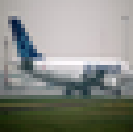
\includegraphics[width=52.5pt,height=52.5pt]{figures/assets/ORIGINAL_GAUSSIAN.png}};
%Image [id:dp988855448482646] 
\draw (188.33,176) node  {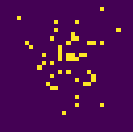
\includegraphics[width=52.5pt,height=52.5pt]{figures/assets/MASK_GAUSSIAN.png}};
%Image [id:dp22673392822113958] 
\draw (309.67,103.67) node  {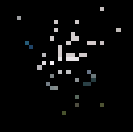
\includegraphics[width=52.5pt,height=52.5pt]{figures/assets/RESULT_GAUSSIAN.png}};
%Curve Lines [id:da7064061111049843] 
\draw    (224.33,86.33) .. controls (257.99,82.37) and (227.62,107.16) .. (272.29,100.54) ;
\draw [shift={(273.67,100.33)}, rotate = 171.07] [color={rgb, 255:red, 0; green, 0; blue, 0 }  ][line width=0.75]    (10.93,-3.29) .. controls (6.95,-1.4) and (3.31,-0.3) .. (0,0) .. controls (3.31,0.3) and (6.95,1.4) .. (10.93,3.29)   ;
%Curve Lines [id:da2412457613293979] 
\draw    (224.33,157.67) .. controls (273.83,153.05) and (228.59,124.9) .. (272.96,117.23) ;
\draw [shift={(274.33,117)}, rotate = 171.07] [color={rgb, 255:red, 0; green, 0; blue, 0 }  ][line width=0.75]    (10.93,-3.29) .. controls (6.95,-1.4) and (3.31,-0.3) .. (0,0) .. controls (3.31,0.3) and (6.95,1.4) .. (10.93,3.29)   ;
%Image [id:dp7901210362437346] 
\draw (431,111.33) node  {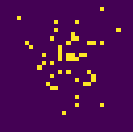
\includegraphics[width=52.5pt,height=52.5pt]{figures/assets/GREEN_GAUSSIAN.png}};
%Image [id:dp9948313666469564] 
\draw (423.67,123) node  {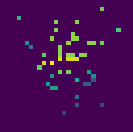
\includegraphics[width=52.5pt,height=52.5pt]{figures/assets/RED_GAUSSIAN.png}};
%Shape: Square [id:dp655934035728707] 
\draw  [color={rgb, 255:red, 255; green, 255; blue, 255 }  ,draw opacity=1 ] (388.67,88) -- (458.67,88) -- (458.67,158) -- (388.67,158) -- cycle ;
%Image [id:dp29091288526835224] 
\draw (417,136) node  {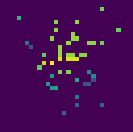
\includegraphics[width=52.5pt,height=52.5pt]{figures/assets/BLUE_GAUSSIAN.png}};
%Shape: Square [id:dp17919766367981604] 
\draw  [color={rgb, 255:red, 255; green, 255; blue, 255 }  ,draw opacity=1 ] (382,101) -- (452,101) -- (452,171) -- (382,171) -- cycle ;
%Image [id:dp6261788477655241] 
\draw (411,148.67) node  {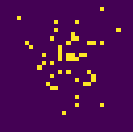
\includegraphics[width=52.5pt,height=52.5pt]{figures/assets/MASK_GAUSSIAN.png}};
%Shape: Square [id:dp8527153376534193] 
\draw  [color={rgb, 255:red, 255; green, 255; blue, 255 }  ,draw opacity=1 ] (376,113.67) -- (446,113.67) -- (446,183.67) -- (376,183.67) -- cycle ;
%Curve Lines [id:da0011889641265926398] 
\draw    (345.67,104.33) .. controls (353.15,122.41) and (361.21,123.58) .. (369.86,125.84) ;
\draw [shift={(371.67,126.33)}, rotate = 195.95] [color={rgb, 255:red, 0; green, 0; blue, 0 }  ][line width=0.75]    (10.93,-3.29) .. controls (6.95,-1.4) and (3.31,-0.3) .. (0,0) .. controls (3.31,0.3) and (6.95,1.4) .. (10.93,3.29)   ;
%Curve Lines [id:da5210657288496086] 
\draw    (224.33,169.67) .. controls (267.89,153.83) and (323.87,157.59) .. (372.2,149.26) ;
\draw [shift={(373.67,149)}, rotate = 169.9] [color={rgb, 255:red, 0; green, 0; blue, 0 }  ][line width=0.75]    (10.93,-3.29) .. controls (6.95,-1.4) and (3.31,-0.3) .. (0,0) .. controls (3.31,0.3) and (6.95,1.4) .. (10.93,3.29)   ;

% Text Node
\draw (162,27.33) node [anchor=north west][inner sep=0.75pt]   [align=left] {Original};
% Text Node
\draw (168.67,123.33) node [anchor=north west][inner sep=0.75pt]   [align=left] {Mask};
% Text Node
\draw (420.67,50.67) node [anchor=north west][inner sep=0.75pt]   [align=left] {$\displaystyle m$};


\end{tikzpicture}
